\documentclass [aspectratio=169]{beamer}
\usetheme{Boadilla}
\usepackage{textpos} % package for the positioning
\usepackage[]{graphicx}
\usepackage{graphicx}
\usepackage{float}
\usepackage{hyperref}
\usepackage{caption}
\usepackage{subcaption}
\usepackage{comment}
\usepackage{algorithm,algpseudocode}
\usepackage[export]{adjustbox}
\usepackage{tikz}
\usepackage{xcolor}
\usepackage{pgfplots}
\pgfplotsset{compat=1.7}
\usetikzlibrary{positioning}
\usetikzlibrary{arrows, shapes, decorations, automata, backgrounds, fit, petri, calc}
\setbeamertemplate{itemize items}[circle]
\setbeamertemplate{enumerate items}[circle]
\setbeamertemplate{itemize subitem}{$\triangleright$}

\newcommand{\notimplies}{\;\not\!\!\!\implies}
\newcommand*{\logofont}{\fontfamily{phv}\selectfont}
\definecolor{uoftblue}{RGB}{6,41,88} % official blue color for uoft

\vspace{1in}
\title[]{DoSS Summer Bootcamp Probability \\ Module 6}
\author[]{Ichiro Hashimoto}
\institute[]{University of Toronto}
\date{July 19, 2024}

% set color
\setbeamercolor{title in head/foot}{bg=white}
\setbeamercolor{author in head/foot}{bg=white}
\setbeamercolor{date in head/foot}{fg=uoftblue}
\setbeamercolor{date in head/foot}{bg=white}
\setbeamercolor{title}{fg=uoftblue}
\setbeamerfont{title}{series=\bfseries}
\setbeamercolor{frametitle}{fg=uoftblue}
\setbeamerfont{frametitle}{series=\bfseries}
\setbeamercolor*{item}{fg=uoftblue}
\setbeamercolor{block title}{bg=uoftblue}
\setbeamercolor{block title}{fg=white}
\setbeamercolor{block body}{bg=uoftblue!5!white}

% set logo at non-title pages
\logo{
\includegraphics[height=0.8cm]{logo_uoft.png}\vspace*{-.055\paperheight}\hspace*{.85\paperwidth}}

% set margin
\setbeamersize{text margin left=10mm,text margin right=10mm}

\newcommand{\mc}{\mathcal}

\begin{document}
{
\setbeamertemplate{logo}{}
\begin{frame}
    \vspace{0.5in}
    \titlepage
    \begin{textblock*}{4cm}(0.5cm,-7.5cm)
        
\includegraphics[width=4cm]{logo_uoft.png}
    \end{textblock*}
    \begin{textblock*}{8cm}(5.0cm,-7cm)
        \huge \color{uoftblue}{$\Bigr\rvert$ \hspace{0.15cm} \textbf{\logofont Statistical Sciences}}
    \end{textblock*}
\end{frame}
}

\begin{frame}{Recap}
Learnt in last module:\\
\vspace{0.1in}
\begin{itemize}
    \item Moments
    \begin{itemize}
        \item Expectation, Raw moments, central moments
        \item Moment-generating functions
    \end{itemize}
    \item Change-of-variables using MGF
    \begin{itemize}
        \item Gamma distribution
        \item Chi square distribution
    \end{itemize}
    \item Conditional expectation
    \begin{itemize}
        \item Law of total expectation
        \item Law of total variance
    \end{itemize}
\end{itemize}
\end{frame}

\begin{frame}{Outline}
\begin{itemize}
    \item Covariance
    \begin{itemize}
        \item Covariance as an inner product
        \item Correlation
        \item Cauchy-Schwarz inequality
        \item Uncorrelatedness and Independence
    \end{itemize}
    \item Concentration
    \begin{itemize}
        \item Markov’s inequality
        \item Chebyshev’s inequality
        \item Chernoff bounds
    \end{itemize}
\end{itemize}
\end{frame}


\begin{frame}{Covariance}
    \textbf{Recall the property of expectation:}\\
    $$
    \mathbb{E}(X + Y) = \mathbb{E}(X) + \mathbb{E}(Y).
    $$
    \uncover<2->{
    \textbf{What about the variance?}\\
    \begin{equation*}
        \begin{aligned}
         Var(X + Y) &= \mathbb{E}(X + Y - \mathbb{E}(X) - \mathbb{E}(Y))^2   \\
         & = \mathbb{E}(X- \mathbb{E}(X))^2 + \mathbb{E}(Y- \mathbb{E}(Y))^2 + 2\mathbb{E}((X- \mathbb{E}(X))(Y- \mathbb{E}(Y)))\\
         & = Var(X) + Var(Y) + 2\underbrace{\mathbb{E}((X- \mathbb{E}(X))(Y- \mathbb{E}(Y)))}_{\text{?}}
        \end{aligned}
    \end{equation*}}
\end{frame}

\begin{frame}{Covariance}
\textbf{Intuition: }\\
A measure of how much $X, Y$ change together.
\uncover<2->{
\vspace{0.1in}
    \begin{block}{Covariance}
    For two jointly distributed real-valued random variables $X, Y$ with finite second moments, the covariance is defined as
    $$
    Cov(X, Y) = \mathbb{E}((X- \mathbb{E}(X))(Y- \mathbb{E}(Y))).
    $$
    \end{block}
    \vspace{0.1in}
    \textbf{Simplification:}
    $$
    Cov(X, Y) = \mathbb{E}(XY) -  \mathbb{E}(X)\mathbb{E}(Y).
    $$
    \vspace{0.5in}}
\end{frame}

\begin{frame}{Covariance}
    \textbf{Properties:}\\
    \begin{itemize}
        \item $Cov(X,X) = Var(X) \ge 0$;
        \item  $Cov(X,a) = 0, \quad a \text{ is a constant}$;
        \item $Cov(X,Y) = Cov(Y,X)$;
        \item $Cov(X + a,Y + b) = Cov(X,Y)$;
        \item $Cov(aX,bY) = abCov(X,Y)$.
    \end{itemize}
    \vspace{0.1in}
    \uncover<2->{
    \textbf{Corollary about variance:}\\
    $$
    Var(aX + b) = a^2 Var(X).
    $$}
\end{frame}

\begin{frame}{Covariance}
    \textbf{Relate covariance to inner product:}\\
\begin{block}{Inner product (not rigorous)}
Inner product is a operator from a vector space $V$ to a field $F$ (use $\mathbb{R}$ here as an example): $<\cdot, \cdot>: V \times V \to \mathbb{R}$ that satisfies:
\begin{itemize}
    \item Symmetry: $<x, y> = <y, x>$;
    \item Linearity in the first argument: $<ax + by, z> = a<x, z> + b<y, z>$;
    \item Positive-definiteness: $<x,x>\ge 0$, and $<x, x> = 0 \Leftrightarrow x = 0$
\end{itemize}
\end{block}
\vspace{0.1in}
\uncover<2->{
\textbf{Remark:}\\
Covariance defines an inner product over the quotient vector space obtained by taking the subspace of random variables with finite second moment and identifying any two that differ by a constant.}
\end{frame}


\begin{frame}{Covariance}
\textbf{Properties inherited from the inner product space}\\
% talk about angle and cauchy schwarz inequality
\vspace{0.1in}
Recall in Euclidean vector space:
\begin{itemize}
    \item  $<x, y> = x^\top y = \sum_{i = 1}^n x_iy_i$;
    \item $||x||_2 = \sqrt{<x,x>}$;
    \item $<x,y> = ||x||_2\cdot ||y||_2 \cos(\theta)$.
\end{itemize}
\vspace{0.1in}
Respectively:
\begin{itemize}
    \item  $<X, Y> = Cov(X, Y)$;
    \item $||X|| = \sqrt{Var(X)}$;
\end{itemize}
\end{frame}

\begin{frame}{Covariance}
\textbf{A substitute for $\cos(\theta)$:}
% become a universal criterion when conducting data analysis.
     \begin{block}{Correlation}
    For two jointly distributed real-valued random variables $X, Y$ with finite second moments, the correlation is defined as
    $$
    Corr(X, Y) = \rho_{XY} = \frac{Cov(X, Y)}{\sqrt{Var(X)\cdot Var(Y)}}.
    $$
    \end{block}
    \vspace{0.1in}
    \uncover<2->{
    \textbf{Uncorrelatedness:}\\
    $$
    X, Y \text{ uncorrelated} \quad \Leftrightarrow \quad Corr(X, Y) = 0.
    $$}
\end{frame}

\begin{frame}{Covariance}
    \begin{block}{Cauchy-Schwarz inequality}
    $$
    {\displaystyle |{Cov} (X,Y)|\leq {\sqrt {Var(X)Var(Y)}}}.
    $$
    \end{block}
    \vspace{0.1in}
\textbf{Proof:}\\
\vspace{2in}
% https://www.probabilitycourse.com/chapter6/6_2_4_cauchy_schwarz.php#:~:text=6.2.,4%20Cauchy%2DSchwarz%20Inequality&text=Let%20us%20state%20and%20prove,Schwarz%20inequality%20for%20random%20variables.&text=For%20any%20two%20random%20variables,some%20constant%20%CE%B1%E2%88%88R.&text=%3DE%5BX2%5D%E2%88%92,2E%5BY2%5D. 
\end{frame}


\begin{frame}{Covariance}
    \textbf{Uncorrelatedness and Independence:}\\
    \vspace{0.1in}
    Observe the relationship:
    $$
    Corr(X,Y) = 0 \quad \Leftrightarrow \quad  Cov(X, Y) = 0 \quad \Leftrightarrow  \quad \mathbb{E}(XY) = \mathbb{E}(X)\mathbb{E}(X)
    $$
    \vspace{0.1in}
    \uncover<2->{
    \textbf{Conclusions:}\\
    \begin{itemize}
        \item Independence $\Rightarrow$ Uncorrelatedness
        \item Uncorrelatedness $\notimplies$ Independence
    \end{itemize}
    \vspace{0.1in}
    \textbf{Remark:}\\
    Independence is a very strong assumption/property on the distribution.}
    % Special case: multivariate normal
\end{frame}

\begin{frame}{Covariance}
    \textbf{Special case: multivariate normal}\\
    \begin{block}{Multivariate normal}
    A $k$-dimensional random vector $\mathbf{X} = (X_1, X_2, \cdots, X_k)^\top$ follows a multivariate normal distribution $\mathbf{X} \sim \mathcal{N}(\boldsymbol{\mu}, \boldsymbol{\Sigma})$, if
    $$
f_{\mathbf {X} }(x_{1},\ldots ,x_{k})={\frac {\exp \left(-{\frac {1}{2}}({\mathbf {x} }-{\boldsymbol {\mu }})^{\mathrm {T} }{\boldsymbol {\Sigma }}^{-1}({\mathbf {x} }-{\boldsymbol {\mu }})\right)}{\sqrt {(2\pi )^{k}|{\boldsymbol {\Sigma }}|}}},
    $$
    where ${\boldsymbol {\mu }}=\mathbb{E} [\mathbf {X} ]=(\mathbb{E} [X_{1}],\mathbb{E}[X_{2}],\ldots ,\mathbb{E} [X_{k}])^\top$, and $[\boldsymbol{\Sigma}]_{i,j} = \Sigma_{i,j} = Cov(X_i, X_j)$.
    \end{block}
    \vspace{0.1in}
  \textbf{Observation:}\\
  The distribution is decided by the covariance structure. 
\end{frame}

\begin{frame}{Covariance}
\vspace{-0.7in}
    \begin{equation*}
       \begin{aligned}
          X_i, i = 1, \cdots k \text{ independent} & \Leftrightarrow f_{\mathbf {X} }(x_{1},\ldots ,x_{k}) = \prod_{i = 1}^k f_{X_i}(x_i)\\
          & \Leftrightarrow \boldsymbol{\Sigma} = I_k \Leftrightarrow Cov(X_i, X_j) = 0, i \neq j.
       \end{aligned}
   \end{equation*}
   \vspace{0.1in}
   \textbf{Example:}\\
   \begin{itemize}
  \only<1>{\item $Corr(X, Y) = 0$}
  \only<2>{\item $Corr(X, Y) = 0.7$}
  \only<3>{\item $Corr(X, Y) = -0.7$}
 \end{itemize}
\begin{overlayarea}{\textwidth}{2cm}
\only<1>{\centering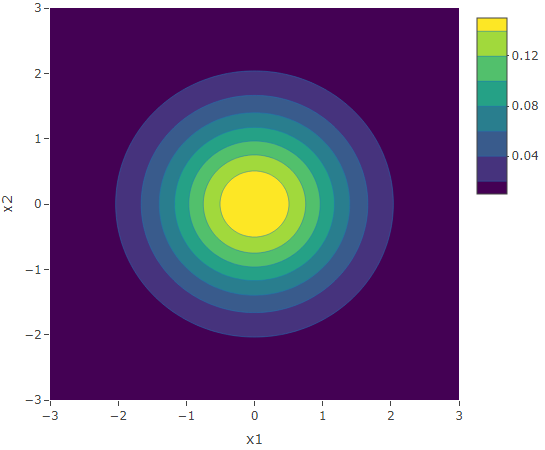
\includegraphics[height=4cm]{CBivariate0corr-1.png}\par}
\only<2>{\centering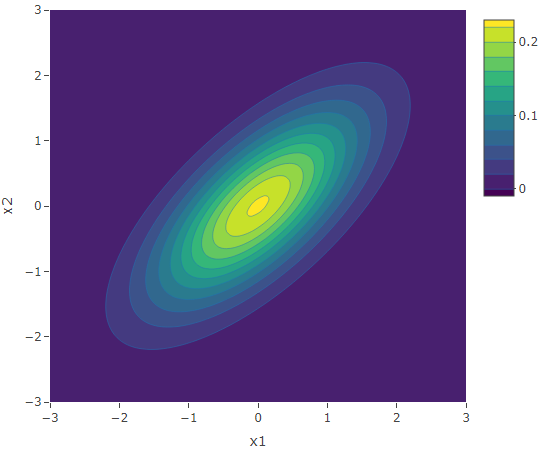
\includegraphics[height=4cm]{CBivariate0.7corr.png}\par}
\only<3>{\centering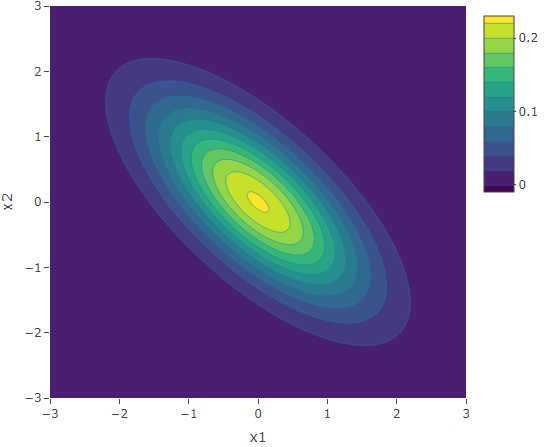
\includegraphics[height=4cm]{CBivariate-0.7corr.png}\par}
\end{overlayarea}
% reference of the figures: https://datasciencegenie.com/3d-contour-plots-of-bivariate-normal-distribution/ 
\end{frame}


\begin{frame}{Concentration}
    % Up to now, we have talked a lot about the probability distribution, and we can actually almost compute everything based on the pdfs and pmfs. But the point of considering expectations, variance and covariance is that, theses things kind of reflect some properties of the distribution, rather than look into details of what is the mathematical expression of the pdf. 
    \textbf{Measures of a distribution:}\\
    \begin{itemize}
        \item $\mathbb{E}(X^k)$, $\mathbb{E}(X), Var(X)$;
        \item $Cov(X,Y)$ and $Corr(X, Y)$.
    \end{itemize}
\vspace{0.1in}
\uncover<2->{
\textbf{Tail probability: $\mathbf{P}(|X| > t)$}\\
\pgfmathdeclarefunction{gauss}{2}{\pgfmathparse{1/(sqrt(2*pi))*exp(-((x)^2)/(2))}}
\begin{figure}
\centering
\begin{tikzpicture}
\begin{axis}[no markers, domain=0:10, samples=100,
axis lines*=left, xlabel=x, ylabel=$f(x)$,
height=4cm, width=8cm,
xtick={-3, -2, 0, 2, 3}, ytick=\empty,
enlargelimits=false, clip=false, axis on top,
grid = major]
\addplot [fill=white, draw=uoftblue, domain=-3:3] {gauss(0,1)} \closedcycle;
\addplot [fill=uoftblue!20, draw=uoftblue, domain=-3:-2] {gauss(0,1)} \closedcycle;
\addplot [fill=uoftblue!20, draw=uoftblue, domain=2:3] {gauss(0,1)} \closedcycle;
\addplot[] coordinates {(-2,0.3) (2,0.3)};
\end{axis}
\end{tikzpicture}
\caption{Probability density function of $\mathcal{N}(0,1)$}
\label{fig:normpdf}
\end{figure}}
\end{frame}

\begin{frame}{Concentration}
\textbf{Concentration inequalities:}\\
\begin{itemize}
    \item Markov inequality
    \item Chebyshev inequality
    \item Chernoff bounds
\end{itemize}
\uncover<2->{
    \begin{block}{Markov inequality}
    Let $X$ be a random variable that is non-negative (almost surely). Then, for every constant $a>0$,
$$
\mathbb{P}(X\geq a)\leq {\frac {\mathbb{E} (X)}{a}}.
$$
    \end{block}
    \textbf{Proof:}\\
    \vspace{0.6in}}
\end{frame}

\begin{frame}{Concentration}
\begin{block}{Markov inequality (continued)}
    Let $X$ be a random variable, then for every constant $a>0$,
$$
\mathbb{P}(|X|\geq a)\leq {\frac {\mathbb{E} (|X|)}{a}}.
$$
    \end{block}
\vspace{0.1in}
\textbf{A more general conclusion:}\\
\begin{block}{Markov inequality (continued)}
    Let $X$ be a random variable, if $\Phi(x)$ is monotonically increasing on $[0, \infty)$, then for every constant $a>0$,
$$
\mathbb{P}(|X|\geq a) = \mathbb{P}(\Phi(|X|)\geq \Phi(a)) \leq {\frac {\mathbb{E} (\Phi(|X|))}{\Phi(a)}}.
$$
    \end{block}
\end{frame}

\begin{frame}{Concentration}
    \begin{block}{Chebyshev inequality}
    Let $X$ be a random variable with finite expectation $\mathbb{E}(X)$ and variance $Var(X)$, then for every constant $a>0$,
    $$
    \mathbb{P}(|X-\mathbb{E}(X)|\geq a) \leq {\frac {Var(X)}{a^2}},
    $$
    or equivalently,
    $$
    \mathbb{P}(|X-\mathbb{E}(X)|\geq a\sqrt{Var(X)}) \leq {\frac {1}{a^2}}.
    $$
    \end{block}
    \vspace{0.1in}
    \textbf{Example:}\\
    Take $a = 2$, $$
    \mathbb{P}(|X-\mathbb{E}(X)|\geq 2\sqrt{Var(X)}) \leq {\frac {1}{4}}.
    $$
\end{frame}


\begin{frame}{Concentration}
    \begin{block}{Chernoff bound (general)}
     Let $X$ be a random variable, then for $t \ge 0$, 
     $$
     {\mathbb{P}(X\geq a)=\mathbb{P}(e^{t\cdot X}\geq e^{t\cdot a})\leq {\frac {\mathbb{E}\left[e^{t\cdot X}\right]}{e^{t\cdot a}}},}
     $$
     and 
     $$
     \mathbb{P}(X\geq a) \le \inf_{t \ge 0}{\frac {\mathbb{E}\left[e^{t\cdot X}\right]}{e^{t\cdot a}}}.
     $$
    \end{block}
    \vspace{0.1in}
    \textbf{Remark:}\\
    This is especially useful when considering $X = \sum_{i =1}^n X_i$ with $X_i$'s independent,
    $$
    {\mathbb{P}(X\geq a)\leq \inf _{t\geq 0}{\frac {\mathbb{E} \left[\prod _{i}e^{t\cdot X_{i}}\right]}{e^{t\cdot a}}}=\inf _{t\geq 0}e^{-t\cdot a}\prod _{i}\mathbb{E} \left[e^{t\cdot X_{i}}\right].}	
    $$
\end{frame}

\begin{frame}{Problem Set}
    \textbf{Problem 1:}  Let
    $$f_{X, Y}(x, y)= \begin{cases}2 & 0 \leq y \leq x \leq 1 \\ 0 & \text { otherwise }\end{cases},
    $$
    compute $Cov(X, Y)$.\\
    % https://www.cs.cmu.edu/~psarkar/sds321/lecture19-new.pdf 
    \vspace{0.1in}
     \textbf{Problem 2:} For $X \sim \mathcal{N}(0,1)$, compute the Chernoff bound.
     % https://ai.stanford.edu/~gwthomas/notes/concentration.html 
    \vspace{0.1in}\\
\end{frame}



\end{document}
